% Idee: Känguru / Sandra Schumann
% Tekst: Sandra Schumann

\documentclass[a4paper,11pt]{article}
\usepackage[et]{../../eio}

\begin{document}
\begin{ol}{\eio}{\ev 10.12.2023}{\yle}{}
\begin{yl}{1}{Juta teekond}{teed}{1 sekund}{10 punkti}

Juta jalutas mööda joonisel näidatud teid. Ta liikus alati vasakult paremale, mitte kunagi paremalt vasakule. Igal teelahkmel oli tal edasi liikumiseks kaks võimalust, millest ta valis ühe.

\begin{center}
  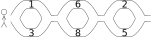
\includegraphics{juta}
\end{center}

Juta kirjutas järjest üles oma teele jäävad arvud.

Kirjuta programm, mis saab kolm arvu ja teeb kindlaks, kas Juta võis need arvud sellises järjekorras üles kirjutada.

\sis Sisendis on kolm rida, igaühel üks täisarv. Esimesel real on arv, mille Juta kirjutas üles esimesena. Teisel real on arv, mille ta kirjutas üles teisena. Kolmandal real on arv, mille ta kirjutas kolmandana. Kõik sisendis olevad arvud on lõigust $0 \ldots 100$.

\val Väljundisse kirjutada üksainus sõna: \verb|JAH|, kui Juta võis antud arve antud järjekorras kohata, ja \verb|EI|, kui see on võimatu. Vastus väljastada suurtähtedega.

\nde[0]{3cm}{3cm}

Arvud 1, 8 ja 5 võivad olla Juta teele jäänud arvud: selleks pidi Juta oma teekonnal kõigepealt liikuma mööda ülemist haru, järgmiseks mööda alumist haru ja viimaseks samuti mööda alumist haru.

\nde[1]{3cm}{3cm}

Arvud 2, 18 ja 85 ei saa olla Juta teele jäänud arvud.

\mrk Pane tähele, et sinu programm ei tohi väljastada mitte midagi muud peale vastuse. Näiteks tekst ``Sisesta esimene arv'' ajab hindamisprogrammi segadusse ja nii võivad ka muidu õige lahenduse eest punktid saamata jääda.

\end{yl}
\end{ol}
\end{document}
